\documentclass[12pt, a4paper]{article}
\usepackage{../notesheets}
\usepackage{tkz-euclide}
%%%%%%%%%%%%%%%%%%%%%%%%%%%%%%%%%%%%%%%%%%%%%%%%%% 
\author{Math 1220}
\title{Vox Populi Midterm 1 Review (Spring 2018)}
\date{}

\begin{document}
\maketitle
%\nameline
%%%%%%%%%%%%%%%%%%%%%%%%%%%%%%%%%%%%%%%%%%%%%%%%%%
\vspace{-0.3in}
\textbf{Sketching Level Curves.} To sketch level curves of \(f(x,y) =
c\) for some constant \(c\), sketch the locus of all points in the
\(xy\)-plane that satisfy the equation.
\begin{ex}
  Sketch the level curves of the function \(f(x,y) = 4x+6y\)
  corresponding to \(z = -2, -1, 0, 1, 2\).
\end{ex}
%\vspace{-2.2in}
\textbf{Volumes and Areas.} If it is not given, half the battle is
finding the right region to integrate! Recall the ``general method''
for finding where a region bounded by curves is. If a region is
bounded by curves \(y = f(x)\) and \(y = g(x)\), solve \(f(x) = g(x)\)
and figure out which function is bigger on each side of the zeros.
\begin{ex}
  Find the volume of the solid of revolution obtained by revolving the
  region bounded by the curves \(y=e^x\) and \(y=x^2+\frac{1}{2}\)
  from \(x=0\) to \(x=1\).
\end{ex}
%\vspace{-2.2in}
\textbf{Using Trig Identities.} The study guide says, ``Because the
ordered pair \((\cos \theta, \sin \theta)\) lies on the unit circle
for which \(x^2+y^2=1\) is an equation, we obtain \emph{the
  fundamental trig identity} \[
  \cos^2 \theta + \sin^2 \theta = 1
\]
You are expected to know the preceding identity as well as the
following quick corollaries:\[
  1+\tan^2 \theta = \sec^2 \theta \text{ and } \cot^2 \theta + 1 =
  \csc^2 \theta
\]
where the former is obtained from the fundamental trig identity by
dividing both sides by \(\cos^2\) and the latter is obtained by
dividing both sides by \(\sin^2 \theta\).'' Why does it say this?
Consider the following question from practice exam S16.
\begin{ex}
  Compute the integral \(\int \cos(x)(1 - \cos^2(x))^{10} \dx\).
\end{ex}
%\vspace{-2.2in}
Or this question from practice exam F16
\begin{ex}
  Prove the identity \(\tan^2 \theta - \sin^2 \theta = \sin^2 \theta
  \tan^2 \theta\) by starting with the expression \(\tan^2 - \sin^2
  \theta\) on the left and showing how it can be transformed, using
  definitions and known identities, into the expression on the right. 
\end{ex}
%\vspace{-2.2in}
\textbf{Trig Related Rates.} The study guide says ``know how to solve related rates problems.''
\begin{ex}
  (Textbook 12.3 exercise 63). A police cruiser hunting for a suspect
  pulls over and stops at a point \(20\) ft from a straight wall. The
  flasher on top of the cruiser revolves at a constant rate of
  \(90^\deg /\)sec, and the light beam casts a spot of light as it
  strikes the wall. How fast is the spot of light moving along the
  wall at a point \(30\) ft from the point on the wall closest to the
  cruiser. \\
  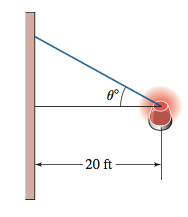
\includegraphics[scale=0.6]{images/police-cruiser}
\end{ex}
%\vspace{-2.2in}
\textbf{Solving problems with given info.} You can get questions where
you are given some information you need and then asked to solve a question.
\begin{ex}
  (F17 8). Suppose that \(f\) is twice differentiable with continuous second
  derivative. The following table gives some values of \(f\) and \(f'\).\[
  \begin{tabular}{|c|c|c|c|c|c|c|c|c|}
    \hline \(x\)&-1&0&1&2&\(e\)&3&5&\(e^2\)\\
    \hline \(f(x)\)&3&-1&7&1&5&\(e^2\)&5&0\\
    \hline \(f'(x)\)&1&-3&4&2&0&-5&11&3\\
    \hline
  \end{tabular}
\]
Use the table above to compute the following. If there is not enough
information to solve the problem, write ``Not Enough Info''.
\begin{enumerate}
\item \(\int_{-1}^2 \frac{f'(x)}{f(x)^2} \dx\)
\item \(\int_0^5 xf''(x)\dx\)
\end{enumerate}
\end{ex}
%\vspace{-2.2in}
\textbf{Unfamiliar word problems.} Do not worry! You know enough to
solve unfamiliar problems.
\begin{ex}
  (F17 11). A pulse traveling along a string can be modeled by the
  equation \[
    u(x,t) = \sin(x-vt)
  \]
  where \(u\) represents the amplitude of the wave, \(x\) is the
  position of the string, \(t\) is the time, and \(v\) is the speed of
  the pulse.
  \begin{enumerate}
  \item Find \(\frac{\partial^2 u}{\partial t^2}\) and
    \(\frac{\partial^2 u}{\partial x^2}\)
  \item We say that \(u\) satisfies the \emph{wave equation} if
    \(\frac{\partial^2 u}{\partial t^2} = v^2 \frac{\partial^2
      u}{\partial x^2}\). Using (a), does \(u(x,t)\) satisfy the wave
    equation?
  \item (Extra; my own.) Sketch level curves for \(u(x,t) = -1, 0, 1\)
    when \(v=1\).
  \end{enumerate}
\end{ex}
%\vspace{-2.2in}
Remember that partial derivatives can also be mixed!
\begin{ex}
  (S16 2). Consider the function \(f(x,y) = \sin(y^3-x)+e^{xy}\). Find
  \(\frac{\partial^2 f}{\partial x \partial y}\).
\end{ex}
%\vspace{-2.2in}
Finally, you can be asked to combine your knowledge in new ways.
\begin{ex}
  (S16 7). Let \(f(x) = \frac{1}{2} \sin^2(x)\) and \(g(x) =
  \frac{1}{2}\cos(x)\). Find the \(x\)-coordinates of all the points
  where the graphs of \(f\) and \(g\) have parallel tangent
  lines. Hint: parallel lines have the same slope.
\end{ex}
%%%%%%%%%%%%%%%%%%%%%%%%%%%%%%%%%%%%%%%%%%%%%%%%%% 
\end{document}
